\subsubsection{48V Speisung}
\label{subsubec:48V Speisung}

\paragraph{Problemstellung}\mbox{}\\

Der Motor wird mit einer Spannung von 48V betrieben. Dies ist zugleich auch die höchste verwendete Speisespannung. Um diese Speisung gewährleisten zu können, wird ein fertiges Netzteil gemäss  \textcolor{red}{\textbf{Fachbericht 5}} eingesetzt.

\paragraph{Schema}\mbox{}\\

Es wurde im Projekt 5 entschieden, dass die 48V Speisung extern als fertiges Netzteil eingekauft wird. Somit entfällt das Schema für diesen Speisungsteil.  

\begin{figure}[h!]
	\centering
	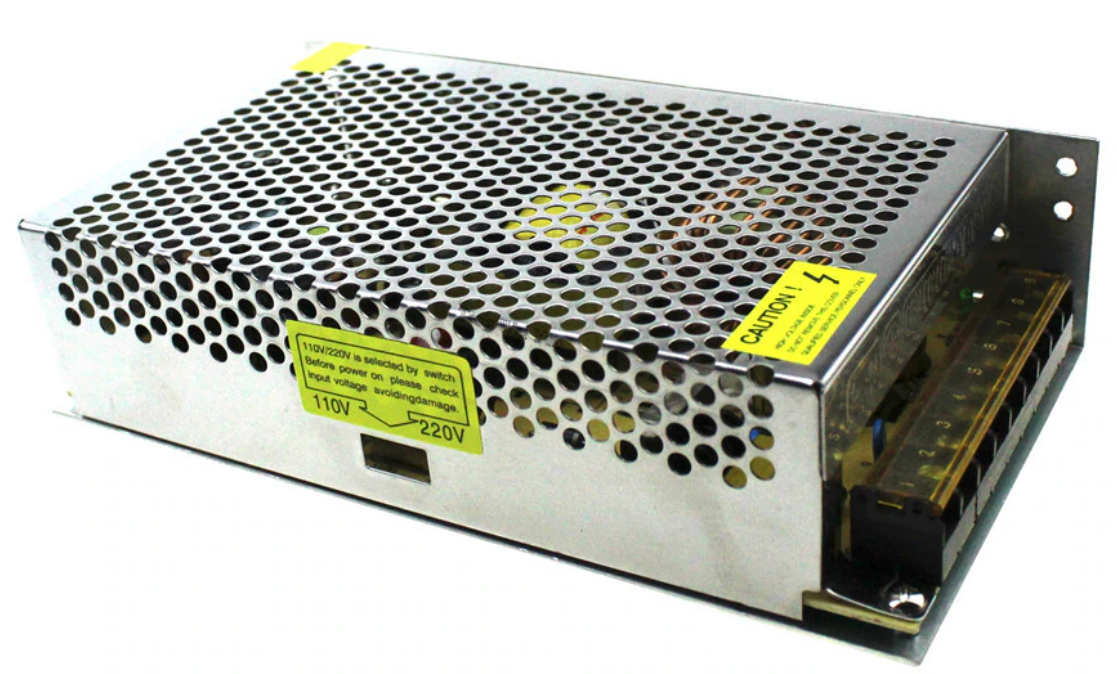
\includegraphics[width=0.8\textwidth]{graphics/Netzteil_48V.png}
	\caption{Anschauungsbild des 48V Netzteils}
	\label{fig:Netzteil_48V}
\end{figure} 


\paragraph{Funktionsbeschrieb}\mbox{}\\

Es musste jedoch unbedingt eine Leistungsabschätzung gemacht werden. Auch diese wurde im Projekt 5 durchgeführt. Unter Berücksichtigung der Schaltungsteile welche noch im Projekt 6 ergänzt werden, wurde dieses dann ausgewählt und eingekauft. Die Leistungsabschätzung kann im \textcolor{red}{\textbf{Fachbericht 5}} eingesehen werden. 